\subsection{Motivation for optimisation approach}
Most approaches to designing Bézier polynomial-based virtual constraints for a bipedal robot can be classed in one of three categories; \textit{manual design}, \textit{sampling} or \textit{optimisation}. Manual design involves a human operator producing the control points directly. Sampling is the utilisation of some method of choosing coefficients in an attempt to span the configuration space, either by random selection or gridding. Optimisation approaches choose coefficients which minimise some cost function under particular constraints.

Manual design approaches are not favourable since they are expensive and inefficient in comparison to automatic generation of virtual constraints. Sampling methods, while much faster at generating a single virtual constraint than manual generation, suffer from the \textit{curse of dimensionality}. That is, in order for a sampling method to produce the same density of coverage, the number of samples required increases exponentially with the number of dimensions. Using a brute-force sampling approach produces many redundant primitives which exhibit similar net changes in the mechanical energy of the walker and paths of the end of the swing leg.

This redundancy increases the the memory required to store the virtual constraint library and the computational requirements of both its generation and use in real time. An optimisation approach attempts to find the best virtual constraint subject to particular requirements, e.g. beginning and final conditions. Therefore, the utility of single constraint optimisation is to avoid the large amount of redundancy involved in the sampling approach. Clearly, single constraint optimisation is itself not sufficient to produce a library of primitives; see Section \ref{sec:lib}.

\subsection{Definition of optimality}
As with most physical systems, there are competing definitions of optimality in the case walking robots; {\color{red}<insert literature references to competing definitions>}.

The definition of optimality chosen for the purposes of producing the virtual constraint library is as follows:
\emph{The optimal virtual constraint for a given start and end configuration and kinetic energy gain or loss is the one which requires the minimum input energy to maintain.}

We note that the relationship between torque and electrical energy in conventional DC motors is typically approximated by the following equation: \cite{??}
\begin{equation} \label{eqn:motorenergy}
	E(t) = \int\limits_0^t u(s)^2 ~ ds
\end{equation}

However, since the partial solution of the zero dynamics is in terms of $\theta$ rather than time, this is not a convenient cost function. Therefore, we assume that $\theta$ progresses reasonably steadily on the interval $[\theta^+,~\theta^-]$ and thus the cost function
\begin{equation}
	J = \int\limits_{\theta^+}^{\theta^-} u_c(\theta) ~ d\theta
\end{equation}
approximates Equation \ref{eqn:motorenergy} evaluated over the virtual constraint.

\subsection{Validity of convex optimisation approach}
The decision variables for the purpose of optimisation are the Bézier coefficients $\alpha$. Since the formulation of the cost function $J$ is not linear or quadratic in these decision variables, the optimisation problem becomes more complex; see Section \ref{sec:nonlinopt}. Linear and quadratic techniques are not immediately applicable to the nonlinear case, leaving two alternatives; gridding approaches and nonlinear programming. Gridding approaches in optimisation are subject to the same limitations described above; indeed, if the advantage of optimisation is to avoid using gridding, then such an approach is clearly a poor choice. However, nonlinear programming will only produce reasonable results under certain conditions.

It is not possible to determine \textit{a priori} that an optimisation is well-formed, that is, will result in a valid solution. Furthermore, for nonlinear optimisation to produce favourable results, the cost function must be convex or near-convex close to the initial estimate. It is therefore of significant interest to determine how close the cost function is to being convex. For the two-link compass gait walker, it is possible to produce such a verification, since we can formulate an optimisation with only two decision variable,s which is easily visualised. In Figure \ref{fig:cggridtorque}, we see that gridding the two decision variables produces a surface that appears to be well-behaved and convex. It is reasonable to suggest that this is generalisable to higher degree constraints with more decision variables for the compass-gait robot.

\begin{figure}
	\centering
	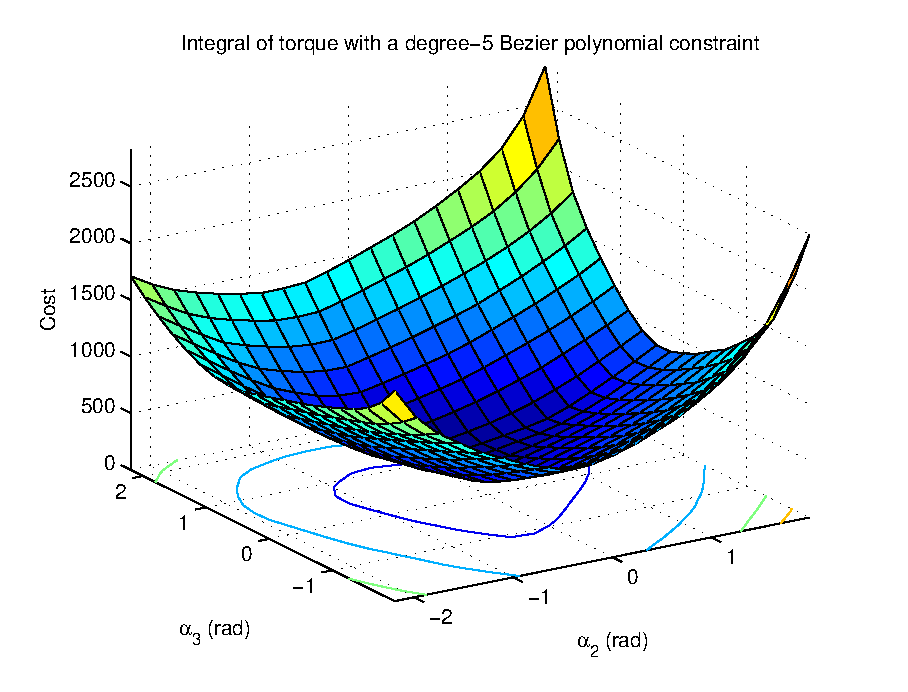
\includegraphics[width=0.8\linewidth]{4VirtConstLib/CGgrid.eps}
	\caption{Cost function of a two decision variable compass-gait optimisation}
	\label{fig:cggridtorque}
\end{figure}

In the case of higher-DOF walking models, it becomes more difficult to confirm near-convexity or even that the cost function is well-behaved. Taking slices, where we choose two decision variables over which to grid and fix all others, allows us to develop some intuition, see Figure \ref{fig:5lslice1} and \ref{fig:5lslice2}. We note that in these slices, the cost function again appears to be well-behaved and near-convex. On the basis of this evidence, it appears to be reasonable to assume that the convex optimisation approach will produce valid results that are near-optimal.

\subsection{Optimisation method}
\subsubsection{Decision variables and constraints}
While the objective of single constraint optimisation is to produce an optimum VC independent of any other virtual constraints in the library, it is important to formulate the optimisation problem in a manner which enables a useful library to be produced. The motion primitive library is intended to contain VCs which span the configuration space of the robot's natural walking as well as including a range of mechanical energy additions and subtractions to facilitate walking over uneven terrain. Therefore, it seems clear that each single constraint optimisation should be formulated subject to constraints on the start and end configurations of the footstep, along with a prescribed energy gain or loss.

Since the potential energy change is prescribed by the start and end conditions, it is convenient to formulate the optimisation using kinetic, rather than total mechanical, energy. The change in kinetic energy $\Delta$KE from one footstep to the next could be calculated with respect to numerous reference points. A simple and obvious choice is to define $\Delta$KE as the change in kinetic energy from $\theta_\alpha^+ \rightarrow \theta_\beta^+$, with $\beta$ being the constraint which follows $\alpha$.

Recall from Section \ref{sec:bezconstraints} that in order to be physically realisable, a VC must satisfy a number of conditions. The latter conditions were concerned only with the single VC, however the \textit{invariance conditions}, \ref{item:configinvariance} and \ref{item:velinvariance}, place restrictions on the admissibility of a primitive on the basis of the VC which preceded it. The first condition is not of great concern in the construction of a single primitive, since the responsibility of ensuring coverage of start and final configurations is deferred to the library generation. However, it is important to consider the latter condition when generating a single constraint, since in order for the library to be useful, any VC which has an initial configuration which matches the final configuration of a constraint through the impact map should be a valid choice of successor. This requires that the slope of all constraints at the end point for any given final configuration is identical. A reasonable choice to satisfy this condition is to enforce that the final slope must be zero for all constraints. This has the additonal advantage of making the constraints more robust to errors in ground height perception.

When formulating an optimisation, it is advantageous to minimise the number of decision variables, if all else is considered static, since this reduces the evaluation time. This is particularly true for variables which are subject to constraints. It is notable that fixing the start and end configuration of the constraint along with enforcing zero slope at the final configuration fixes the four outermost columns of $\alpha$. We therefore consider these fixed and exclude them as decision variables. The optimisation variables therefore take the form given in Table \ref{tab:optDecVars}. Note that the conditions in Section \ref{sec:bezconstraints} are all concerned with those four outermost columns of $\alpha$, therefore in the single VC optimisation, these conditions are not applicable.

\begin{table}
	\centering
	\begin{tabular}{c | c | c | c}
		            Variable             & Generated                     & Decision Variable & Optimisation constraint \\ \hline
		   $\theta^+$ and $\theta^-$     & Supplied                      & No                & No                      \\
		   $\alpha_0$ and $\alpha_N$     & Supplied                      & No                & No                      \\
		         $\alpha_{N-1}$          & Set to $\alpha_N$             & No                & No                      \\
		           $\alpha_1$            & From \ref{item:velinvariance} & No                & No                      \\
		$\alpha_2, \ldots, \alpha_{N-2}$ & Optimisation                  & \textbf{Yes}      & No                      \\
		           $\Delta$KE            & Supplied                      & No                & \textbf{Yes}            \\
	\end{tabular}
	\caption{Variables involved in the single VC optimisation}
	\label{tab:optDecVars}
\end{table}

\subsubsection{Nominal initial velocity}
The torque required to maintain a virtual constraint is not only dependent on the configuration path, but also the velocity. VCs prescribe the configuration path and constrain the velocity to be a function of the initial phase variable velocity. As a result, the torque required to maintain a virtual constraint is a function of the initial velocity. In addition, $\Delta$KE is affine in the square of the initial phase variable velocity. It is therefore necessary to formulate a \textit{nominal initial velocity}, $\dot{\theta}_*$. We assume that in practice, the constraint will be chosen with initial velocities close to $\dot{\theta}_*$ and should therefore be near-optimal. Under that assumption, the change in kinetic energy should be close to the prescribed $\Delta$KE, however, this is less important since the fixing of $\Delta$KE is in service of producing a rich library.

Choosing a nominal velocity for each constraint is non-trivial. Fixing $\dot{\theta}_*$ is not appropriate, since constraints which add kinetic energy to the system are likely to be used when the robot is moving more slowly than for constraints which remove energy. There are several different formulations which are suited to VCs exhibiting certain characteristics. We note that the post impact velocity is calculable with $\Delta_{\dot{\theta}}$ as defined in Equation \ref{eqn:Delthd}:
\begin{subequations}
	\begin{align}
	\left(\dot{\theta}^-\right)^2 &= \Gamma(\theta^-)\dot{\theta}_*^2 + \Psi(\theta^-) \\
	\dot{\theta}^+ &= c\Delta_{\dot{\theta}}\dot{\theta}^-
	\end{align}
\end{subequations}

For \textbf{periodic constraints}, i.e. primitives which neither add nor subtract kinetic energy, the clear choice of nominal velocity is the periodic velocity; the velocity for which the output of the impact map $\dot{\theta}^+$ is equal to the initial velocity $\dot{\theta}_*$. Equating $\dot{\theta}^+$ and $\dot{\theta}_*$, we obtain:
\begin{equation}
	\dot{\theta}_{*,p}^2 = \frac{\Psi(\theta^-)}{(c\Delta_{\dot{\theta}})^{-2} - \Gamma(\theta^-)}
\end{equation}
For \textbf{energy-subtractive constraints}, for which $\Delta$KE $<0$, the choice of nominal velocity is less elegant. Assuming that the robot should never come to a stop or fall back, the energy reduction should result in further constraints being feasible. In order to avoid using any data external to the constraint, the nominal velocity is set to be that which achieves $\dot{\theta}^+ = \lambda\dot{\theta}_{0,c}$, where $\lambda$ is some fixed ``factor of safety''.
Equating $\dot{\theta}^+$ with $\lambda\dot{\theta}_{0,c}$:
\begin{equation}
	\dot{\theta}_{*,\Delta\mathrm{KE}^-}^2 = \frac{(c\Delta_{\dot{\theta}})^{-2}\left(-\lambda^2\frac{ \Psi(\theta_c)}{ \Gamma(\theta_c)}\right) - \Psi(\theta^-)} {\Gamma(\theta^-)}
\end{equation}
For \textbf{energy-additive constraints}, for which $\Delta$KE $>0$, the key issue of importance is that the virtual constraint itself is feasible, since the next primitive will have additional kinetic energy. Therefore, using the same factor of safety $\lambda$ as before, we produce:
\begin{equation}
	\dot{\theta}_{*,\Delta\mathrm{KE}^+}^2 = -\lambda^2\frac{ \Psi(\theta_c)}{ \Gamma(\theta_c)}
\end{equation}

\subsection{Implementation}
The single VC implementation was achieved using MATLAB's constrained nonlinear programming function \mcode{fmincon}. This uses an interior point method to seek local minima in the cost function subject to the given constraints. For each set of test values for the decision variables, the partial solution ($\Gamma(\theta)$ and $\Psi(\theta)$) was evaluated by producing a grid of $\theta$ values in $[\theta^+, \theta^-]$. The cost was calculated using trapezoidal integration on the resulting torque values. Since $\Delta$KE also relies upon the partial solution, it was held persistently in a helper function and only recalculated upon differing decision variables, to avoid inefficient recalcuation.

Other than the $\Delta$KE constraint, no other constraints or bounds were placed upon the coefficients. This is due to the well-behaved nature of the problem; large deviatons always cost more in terms of input torque than small ones. It therefore makes little sense to arbitrarily constrain the decision variables.

The \mcode{optimiseConstraint} function takes as arguments the start and end configurations of the constraint, the desired change in kinetic energy, and the degree of the desired Bézier polynomial. It returns the start and end values of the phase variable $\theta^+$, $\theta^-$ and the Bézier coefficients $\alpha$. These are sufficient to define the virtual holonomic constraint, however, for convenience, it also returns the calculated values of the partial solution at $\theta^+$, $\theta^-$ and $\theta_c$.